\documentclass{article}

\usepackage{hyperref}
\usepackage[a4paper, margin=1in]{geometry}
\usepackage{cite}
\usepackage{upquote}
\usepackage{parskip}
\usepackage{tikz}
\usepackage{textcomp}

\tikzstyle{plain} = [rectangle, rounded corners, text centered, draw=black]
\tikzstyle{trusted} = [rectangle, rounded corners, text centered, draw=black, fill=red!20]
\tikzstyle{untrusted} = [rectangle, rounded corners, text centered, draw=black, fill=yellow!20]
\tikzstyle{arrow} = [thick,->,>=stealth]

\title{Kerberos-based single sign-on with delegation for web applications}
\author{Daniel Carter}
\date {\today}

\begin{document}
\maketitle

\section{Introduction}

\subsection{Web application security}
Many web applications are built around a database, which is used by the application framework to store user data and load it for display to the user. In general, the user logs in using a username and password (which is checked by the web app framework itself), and the application then makes database queries on the user's behalf, processes the results, and displays them to the user in a suitable way.

In this scenario, the application framework has the ability to read and write arbitrary data in the database, and the only thing which prevents a malicious user from accessing data which they are not authorised to read is the application code itself. This is potentially problematic, since web app authors are often not security experts and may accidentally cause data to be visible to the wrong users. Some examples of how this can occur include:

\begin{itemize}
\item
  \textbf{SQL injection}, a form of command injection attack (which are currently number 1 in the OWASP \textit{Top 10 Web Application Security Risks} list\cite{OWASP10}). This occurs when an application uses a template database query such as
\begin{verbatim}
SELECT * FROM records WHERE username='$user';
\end{verbatim}
and replaces \verb+$user+ with a string that the user provides. However, with insufficient checking of parameters, a user can supply a string such as
\begin{verbatim}
' OR 1=1; --
\end{verbatim}
resulting in a total query of
\begin{verbatim}
SELECT * FROM records WHERE username='' OR 1=1; --';
\end{verbatim}
which returns the records of all users (since \verb+1=1+ is always true).

\item
  \textbf{Master password leakage}, which enables any user to arbitrarily read and write from the database. Since the web app itself has these capabilities, it usually has a single username and password which it uses to authenticate with the database, and these are usually stored in a simple configuration file. If the webserver is misconfigured such that the configuration file is visible over the internet, or if the file is accidentally checked into a public source control repository, an attacker can read this file, connect to the database server and read out all the data.

\end{itemize}

As well as being commercially and reputationally damaging, unauthorised access to data can result in severe legal penalties: the Data Protection Act 2018 specifies a fine of up to 2\% of a company's global turnover (or 10 million Euros, if that is greater) may apply in cases of unauthorised disclosure of personal data\cite{GDPR}. Developing technologies that mean the web app does not have to be trusted with all data can significantly reduce the risk of these types of disclosure.

The following diagram represents an example of a typical current setup, and the problems that can be caused if an SQL injection vulnerability is present:

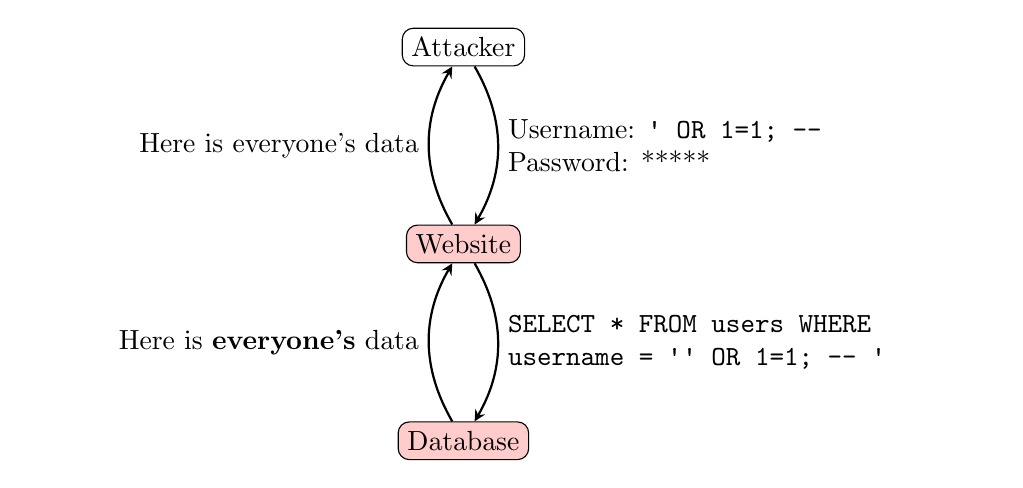
\begin{tikzpicture}[node distance=2.5cm]
  \node (user) [plain] {Attacker};
  \node (webserver) [trusted, below of=user] {Website};
  \node (database) [trusted, below of=webserver] {Database};

  \draw [arrow, bend left] (user) edge node[right] {\parbox{0.5\textwidth}{Username: \texttt{\textquotesingle \ OR 1=1; --} \\ Password: *****}} (webserver);

  \draw [arrow, bend left] (webserver) edge node[right] {\parbox{0.5\textwidth}{\raggedright \texttt{SELECT * FROM users WHERE \\ username = \textquotesingle\textquotesingle \ OR 1=1; -- \textquotesingle}}} (database);

  \draw [arrow, bend left] (database) edge node[left] {\parbox{0.4\textwidth}{\hfill Here is \textbf{everyone's} data}} (webserver);
  \draw [arrow, bend left] (webserver) edge node[left] {\parbox{0.4\textwidth}{\hfill Here is everyone's data}} (user);        
\end{tikzpicture}

\subsection{Website Sign-on Systems}
A further disadvantage of having a ``local'' system of checking passwords on each website is that users are then expected to memorise a large number of different passwords, since otherwise a compromise of the password database of one website would allow the attacker to impersonate users on any other website where they had used the same password. Especially where several websites are ``connected'' in some way (e.g.\ by all being associated with the same organisation), a \textit{single sign-on} system can offer significant benefits.

A single sign-on (SSO) system generally consists of an authentication server, which collects a password (or some other security token) from the user and verifies the user's identity. When a user wishes to log on to a site which uses that SSO system, the user is redirected to the authentication server to log in. Assuming the login in successful, the user is redirected back to the site, along with some kind of unforgeable token to indicate that the authentication server has verified the user's identity.

Note that these steps only provide \textbf{authentication} of the user (i.e.\ that the person logging into the site is actually user $X$). \textbf{Authorisation} (i.e.\ checking whether user $X$ is entitled to access the site) must be done separately by the sites themselves.

The University's Raven authentication service is an example of an SSO system; numerous similar systems exist (including OAuth2, which also has the ability to do a form of ``delegation'' to allow one server to request resources from another, on behalf of the user\cite{Oracle-OAuth2}.

\subsection{Project Summary}
This project aims to produce an authentication system for web applications, such that a user can authenticate to a web application using a Kerberos ticket and the web application can use this ticket to obtain the user's data from a database. The overall structure of the authentication process is as shown below, noting that the application itself does not have any other access means of accessing the database, so an attack such as the one depicted above cannot take place.

Since the same KDC can be used for many websites where the users all have a login to the same Kerberos realm, the system also functions as a single sign-on system (using the Kerberos ticket as proof of identity). As detailed in sections 2 and 3, this does \textbf{not} mean that any of the individual websites need to be given access to the user's password, or that they are able to arbitrarily impersonate the user on other systems. The possibility of delegating tickets in a controlled manner means that the website shown can fetch data from the database on behalf of the user, but not from other systems which it has not been authorised to access.

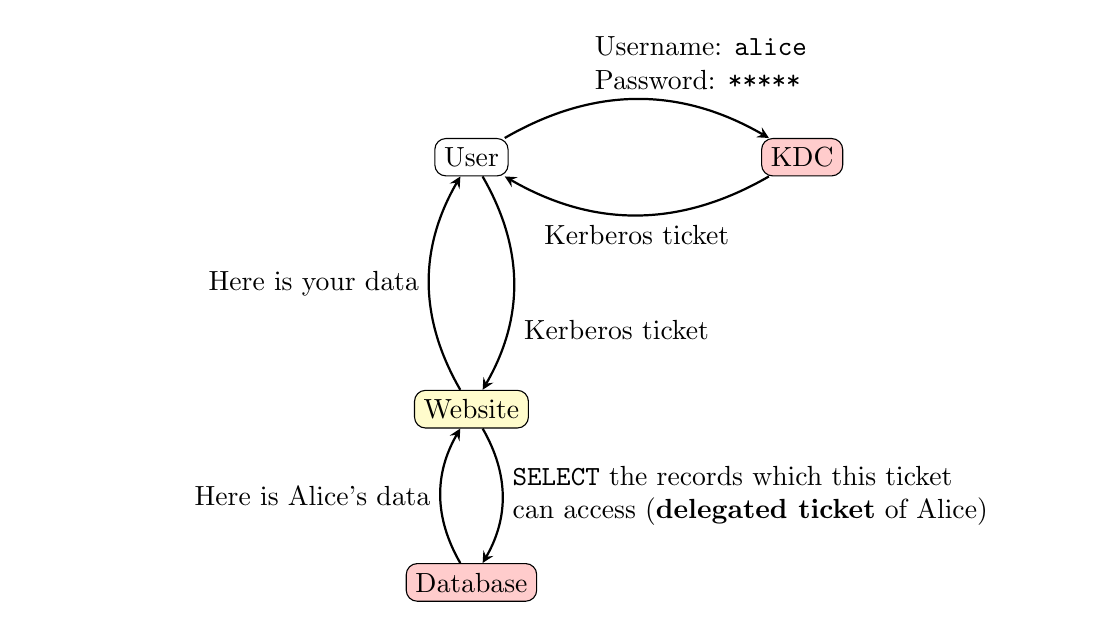
\begin{tikzpicture}[node distance=2.2cm]
  \node (user) [plain] {User};
  \node (webserver) [untrusted, below of=user, yshift=-1cm] {Website};
  \node (database) [trusted, below of=webserver] {Database};
  \node (kdc) [trusted, right of=user, xshift=2cm] {KDC};

  \draw [arrow, bend left] (user) edge node[above, xshift=2.5cm] {\parbox{0.5\textwidth}{Username: \texttt{alice} \\ Password: \texttt{*****}}} (kdc);

  \draw [arrow, bend left] (kdc) edge node[above, yshift=-0.5cm] {Kerberos ticket} (user);

  \draw [arrow, bend left] (user) edge node[right, yshift=-0.6cm] {Kerberos ticket} (webserver);

  \draw [arrow, bend left] (webserver) edge node[right] {\parbox{0.5\textwidth}{\raggedright \texttt{SELECT} the records which this ticket can access (\textbf{delegated ticket} of Alice)}} (database);

  \draw [arrow, bend left] (database) edge node[left] {\parbox{0.4\textwidth}{\hfill Here is Alice's data}} (webserver);
  \draw [arrow, bend left] (webserver) edge node[left] {\parbox{0.4\textwidth}{\hfill Here is your data}} (user);
\end{tikzpicture}

\subsection{Related Work}
The original concept for this project was based on a system developed by Microsoft in IIS 5.0, which added a ``negotiate'' extension to the HTTP protocol for use with Kerberos. This standard is described in RFC 4559\cite{RFC4559} and described a system which allowed a user to log into a web application, from which a suitably equipped application could delegate the ticket to another system such as a database server. This permitted a user to log in to the website without needing a password, in effectively the same way as in the diagram above.

The ``HTTP Negoatiate'' extension was subsequently included in various open-source web browsers. It also has some support in the Apache web server, but this is generally used only to authenticate the user rather than for delegation purposes. The aim of this project is effectively to replicate Microsoft's setup using an open-source web framework (Django) in conjunction with the Apache web server and any client web browser which supports the Negotiate extension.


\section{Preparation}

\subsection{Kerberos}
The Kerberos protocol works based on a system of \textit{tickets}, which are managed by a \textit{Key Distribution Centre} (KDC). The basic requirement of the system is to allow a centralised database of users (for example, the main login directory in an office) who can demonstrate their identity in order to log in to applications and services, but \textit{without} having to store or transmit passwords or other long-term secrets on potentially untrusted machines.

The basic workings of the protocol are as follows:

\begin{itemize}
\item
  A user initiates a session by reqesting a Kerberos ticket from the KDC, authenticating using their password.
\item
  The KDC returns a \textit{ticket-granting ticket} (TGT), and returns it encrypted using the user's password.
\item
  The user decrypts the TGT, and the user's machine can then discard the stored password.
\item
  When the user wants to access a service, they send the TGT back to the KDC along with an identifier for the service which they want to use.
\item
  The TGT grants the user a \textit{service ticket}, which the user then passes on to the service. The service is then able to use that ticket for authentication.
\end{itemize}

The following listing shows a client which has obtained both a TGT and a service ticket. The ticket in the first line (\verb+krbtgt/LOCAL@LOCAL+) is the \textit{ticket-granting ticket} which the client obtained when first authenticating to the KDC, and the second (\verb+HTTP/krbsite.local@LOCAL+) is a \textit{service ticket} to log in to the \verb+HTTP+ service on \verb+krbsite.local+ (i.e.\ to access the web page hosted on that server).

\begin{quote}
\begin{verbatim}
daniel@Daniel-Laptop:~$ klist
Ticket cache: FILE:/tmp/krb5cc_1000
Default principal: dcc@LOCAL

Valid starting     Expires            Service principal
02/04/21 15:36:01  03/04/21 01:36:01  krbtgt/LOCAL@LOCAL
	renew until 03/04/21 15:36:01
02/04/21 15:36:07  03/04/21 01:36:01  HTTP/krbsite.local@LOCAL
	renew until 03/04/21 15:36:01
\end{verbatim}
\end{quote}

\subsection{Kerberos Ticket Delegation}
In addition to use for authentication, Kerberos supports a method of \textit{delegating} tickets. This means that a principal $A$ can pass a ticket to a service $X$ as a means of authentication, and $X$ can pass the ticket on to a third system $Y$ to request resources on the user's behalf.

This is valuable because it means that $X$ can access resources which ``belong'' to $A$, without $X$ needing to have direct access to $Y$. This means that less trust in $X$ is needed (since it does not need privileged access to $Y$), and so the types of attacks discussed above become much less likely.


\section{Implementation}

\subsection{System Structure}
The core of this project is a Django web app, which is able to both perform the necessary setup steps to get the system working and (as a separate component) demonstrate the working of the system.

\subsection{Kerberos Ticket Delegation}
A core aspect of this project is how a ticket can be \textit{delegated} from one server to another, such that the ticket used to log into the web app can be used to authenticate to another system.

\subsubsection{Unconstrained Delegation}
The traditional, and simplest, method for delegation is simply for the user $A$ to pass their ticket-granting ticket to the service $X$. $X$ can now behave as though it were $A$, and access any resources to which $A$ has access by simply presenting $A$'s ticket-granting ticket to the KDC and requesting a suitable service ticket.

In MIT Kerberos, this is achieved by marking service $X$ with the \verb+ok-as-delegate+ flag, which ``hints the client that credentials can and should be delegated when authenticating to the service''\cite{KDC-conf-docs}.

Despite seemingly being no better than $A$ simply giving a password to $X$ (so that $X$ can log in ``as'' $A$ when accessing $Y$), this scheme offers some advantages:

\begin{itemize}
\item
  Kerberos tickets are time-limited, so if $A$ no longer wishes to allow $X$ to access resources, all $A$ has to do is wait for any delegated tickets which $X$ currently holds to expire (and not send any more). This contrasts with passwords which are valid indefinitely and may well not be straightforward to change in a complex corporate network.
\item
  Some limitations are placed on what can be done with the tickets. Although $X$ can use the TGT to get a service ticket to any other system $Y$ that $A$ can access, $Y$ does not automatically have the right to delegate this ticket further. If $Y$ does \textbf{not} have the \verb+ok-as-delegate+ flag set, then $X$ can \textit{access} $Y$ on $A$'s behalf but not allow $Y$ to perform actions for $A$ on some other server $Z$. If $Y$ is not well-trusted, this can be a significant benefit.
\end{itemize}

% Discuss NTLM fallbacks?

While the second of these advantages is significant, it may still not offer enough access control over the network. In particular, $A$ cannot give $X$ the ability to delegate to $Y$ without also giving $X$ the ability to delegate to \textbf{any} other service which $A$ has access to. In many cases this would be too great a risk; it may well be desirable to allow $X$ to fetch $A$'s work documents from $Y$ to display them in a web app, but not to allow $X$ to retreive $A$'s financial records from another system $Z$ within the same Kerberos realm.

In this case, constrained delegation offers a far more controllable method of only services to delegate tickets in particular ways, at the expense of a more complex setup for managing applications.

\subsubsection{Constrained Delegation (S4U2proxy)}
The \textit{Service for User to Proxy} (S4U2proxy) system is an extension to the basic Kerberos setup that allows one service $X$ to obtain a ticket to another service $Y$ (on behalf of a principal $A$) in a controlled manner. Once service $X$ has been marked as ``permitted'' to obtain tickets for service $Y$, it can do so simply by making a request to the KDC, without having any need to know the user's Kerberos password\cite{MS-s4u2}.

Unlike with unconstrained delegation, here the ticket-granting ticket is not passed over to $X$; instead, $X$ is given a service ticket from $A$ as normal (to prove $A$'s identity and that $A$ wishes to connect to $X$). When $X$ needs to access $Y$ on behalf of $A$, $X$ \textit{submits the service ticket} to the KDC. If the permissions in the KDC are set appropriately, it is able to give $X$ a ticket to $Y$ on behalf of $A$.

This requires a more complex setup of permission models in the KDC than simply a list of principals, since the KDC must now decide which services can delegate tickets to which others. The default back-end for MIT Kerberos does not support this, but moving the user data into an LDAP server and using this as the data source allows the relevant \texttt{krbAllowedToDelegateTo} permission to be set on the user\cite{KRB-DELEG}.

In addition to the advantages described above for unconstrained delegation, there are some further advantages here:

\begin{itemize}
\item
  Access control can be almost completely customized. The system can now be set up so that $A$ can log into $X$ and have a Kerberos ticket delegated to $Y$, or log into $P$ and have a ticket delegated to $Q$, but not allow $X$ to delegate to $Q$. There is no simple set of ``privileged'' applications which are allowed to perform (all) delegation, but a customizable set of permissions between systems.
\item
  The number of powerful ticket-granting tickets that are stored in systems on the network is reduced. If an attacker gains access to $X$, the attacker will, at most, get service tickets for all users who have recently logged into $X$ (i.e.\ who have logged in and whose stored tickets have not yet expired), and delegated service tickets to the services which $X$ is allowed to. The attacker does not get a ticket-granting ticket to use on arbitrary applications.
\end{itemize}

\subsubsection{S4U2self}
This description is included here for completeness (because of its similar name) although it is \textbf{not} a true method of delegating tickets.

The Microsoft standard document for S4U2self\cite{MS-s4u2} states that:

\begin{quote}
  The S4U2self extension allows a service to obtain a service ticket to itself on behalf of a user. The user is identified to the KDC using the user's name and realm. Alternatively, the user might be identified based on the user's certificate.
\end{quote}

In effect, Kerberos authentication is bypassed completely and the server $X$ is able to get a ticket for $A$ simply by specifying $A$'s user name. This may be useful in some situations if not all clients can use Kerberos, but it offers a significantly weaker security model (since $X$ can now obtain service tickets for any user) and so if $X$ is compromised then records from all users can be gathered. As the aim of this project is to reduce the amount of trust placed in applications such as $X$, S4U2self is of no use and will not be considered further.

\subsection{SQL Access Control}
As one aspect of the project, the database server must be able to provide the correct set of records to each user without exposing the rest of the table. Since PostgreSQL does not offer the ability to selectively allow a user to query certain rows in a table, this can instead be acheived using stored procedures. However, these are not a standardised construct in SQL, and even within PostgreSQL there are multiple ways to achieve this.

\subsubsection{\texttt{SECURITY DEFINER} functions}
A PostgreSQL function with \texttt{SECURITY DEFINER} in the signature runs ``as'' the user creating the function, regardless of who executes it\cite{postgres-SEC_DEF} (in a similar way to how the \texttt{setuid} bit works in Unix). This allows the database owner to create a function which can read the whole table and when run, perform some check based on the user calling it and return appropriate results.

This approach requires some caution since the \texttt{SECURITY DEFINER} property also redefines the \verb+current_user+ variable (which normally contains the username of the user executing a query) to the user who defined the function, although this can be worked around using \verb+session_user+ instead. It is also not as easily integratable into frameworks such as Django, which are designed to execute queries on tables rather than (effectively) making function calls to an API.

\subsubsection{Use of \texttt{ON SELECT} to redefine selection}
PostgreSQL also allows rules to be created which effectively redefine actions on tables. For example, a rule could be used to replace the default \texttt{SELECT} rule on the table storing file information with one that checked user permissions.

However, this is likely to introduce unnecessary complexity (particularly with ensuring that administrators can still access data as necessary, for example). For these reasons, the PostgreSQL documentation considers it ``better style to write a \texttt{CREATE VIEW} command than to create a real table and define an \texttt{ON SELECT} rule for it''\cite{postgres-CREATE_RULE}.

\subsubsection{SQL views}
These effectively allow a new table to be created out of a view over an existing table. Using syntax such as the following, it is therefore possible to construct a new table which only has the calling user's files visible; the user can then be granted access to this view (which automatically selects files based on their own username) and does not then need to have any access to the original table. For web application purposes, it can be queried just like any other table.

\begin{verbatim}
CREATE VIEW my_files AS
SELECT f.*
FROM files_file f, files_permission p
WHERE f.id = p.file_id
AND p.owner = user;
\end{verbatim}

\section{Evaluation}

\section{Conclusion}

\section*{Bibliography}
\begin{thebibliography}{9}
\bibitem{OWASP10} OWASP \textit{Top 10 Web Application Security Risks} list. \url{https://owasp.org/www-project-top-ten/} (accessed 21/10/2020)

\bibitem{GDPR} Data Protection Act 2018: Section 157 \url{https://www.legislation.gov.uk/ukpga/2018/12/section/157/enacted} (accessed 10/02/2021)

\bibitem{Oracle-OAuth2} Oracle OAuth Guide: API Gateway OAuth 2.0 Authentication Flows \url{https://docs.oracle.com/cd/E50612_01/doc.11122/oauth_guide/content/oauth_flows.html} (accessed 08/04/2021)

\bibitem{RFC4559} Microsoft Corporation (June 2006), \textit{SPNEGO-based Kerberos and NTLM HTTP Authentication in Microsoft Windows} (RFC 4559): \url{https://tools.ietf.org/html/rfc4559} (accessed 04/04/2021)

\bibitem{KDC-conf-docs} MIT Kerberos documentation: \texttt{kdc.conf} \url{https://web.mit.edu/kerberos/www/krb5-devel/doc/admin/conf_files/kdc_conf.html} (accessed 05/04/2021)

\bibitem{MS-s4u2} Microsoft Corporation (May 2014), \textit{Kerberos Protocol Extensions: Service for User and Constrained Delegation Protocol}: \url{https://winprotocoldoc.blob.core.windows.net/productionwindowsarchives/MS-SFU/[MS-SFU]-140515.pdf} (accessed 05/04/2021)

\bibitem{KRB-DELEG}  Kerberos: delegation and s4u2proxy (Simo Sorce, 12/02/2012) \url{https://ssimo.org/blog/id_011.html} (accessed 02/02/2021)

\bibitem{postgres-SEC_DEF} PostgreSQL documentation: \texttt{CREATE FUNCTION} \url{https://www.postgresql.org/docs/current/sql-createfunction.html#SQL-CREATEFUNCTION-SECURITY} (accessed 22/02/2021)

\bibitem{postgres-CREATE_RULE} PostgreSQL documentation: \texttt{CREATE RULE} \url{https://www.postgresql.org/docs/current/sql-createrule.html} (accessed 22/02/2021)

\end{thebibliography}

\end{document}
